\documentclass[aspectratio=169, 11pt]{beamer}
% ============================================================================
% Preambulo compartido para presentaciones Beamer
% Estadistica 2026-II - Pontificia Universidad Javeriana
% Incluir con: % ============================================================================
% Preambulo compartido para presentaciones Beamer
% Estadistica 2026-II - Pontificia Universidad Javeriana
% Incluir con: % ============================================================================
% Preambulo compartido para presentaciones Beamer
% Estadistica 2026-II - Pontificia Universidad Javeriana
% Incluir con: \input{../preambulo_beamer.tex} despues de \documentclass
% ============================================================================

\usepackage[T1]{fontenc}
\usepackage[utf8]{inputenc}
\usepackage[spanish]{babel}
\usepackage{amsmath, amssymb, amsfonts}
\usepackage{booktabs}
\usepackage{graphicx}
\usepackage{tikz}
\usetikzlibrary{shapes.geometric, positioning, arrows.meta, calc}
\usepackage{pgfplots}
\pgfplotsset{compat=1.18}
\usepackage{listings}
\usepackage{xcolor}
\usepackage{hyperref}
\usepackage{multicol}


% --- Tema Beamer (minimalista) ---
\usetheme{default}
\usecolortheme{default}
\usefonttheme{default}
\setbeamertemplate{navigation symbols}{}
\setbeamertemplate{caption}[numbered]
\setbeamertemplate{footline}{%
  \hfill\usebeamerfont{footline}\insertframenumber/\inserttotalframenumber\hspace{1em}\vspace{0.5em}%
}
\setbeamertemplate{itemize items}[circle]
\setbeamertemplate{enumerate items}[default]

% --- Colores institucionales (sutiles) ---
\definecolor{javeriana}{RGB}{0, 62, 105}
\definecolor{javerianalight}{RGB}{0, 105, 170}
\definecolor{codigobg}{RGB}{245, 245, 245}
\definecolor{codigofg}{RGB}{40, 40, 40}
\definecolor{comentario}{RGB}{100, 100, 100}
\definecolor{keyword}{RGB}{0, 100, 150}
\definecolor{string}{RGB}{180, 60, 30}

\setbeamercolor{title}{fg=javeriana}
\setbeamercolor{frametitle}{fg=javeriana}
\setbeamercolor{structure}{fg=javeriana}
\setbeamercolor{block title}{fg=white, bg=javeriana!75}
\setbeamercolor{block body}{bg=javeriana!5}
\setbeamercolor{block title alerted}{fg=white, bg=red!70!black}
\setbeamercolor{block body alerted}{bg=red!5}
\setbeamercolor{block title example}{fg=white, bg=green!40!black}
\setbeamercolor{block body example}{bg=green!5}
\setbeamercolor{item}{fg=javeriana}

\setbeamerfont{title}{series=\bfseries, size=\Large}
\setbeamerfont{frametitle}{series=\bfseries}

% --- Configuracion de listings para R ---
\lstset{
  language=R,
  basicstyle=\ttfamily\footnotesize,
  backgroundcolor=\color{codigobg},
  commentstyle=\color{comentario}\itshape,
  keywordstyle=\color{keyword}\bfseries,
  stringstyle=\color{string},
  numbers=none,
  frame=single,
  rulecolor=\color{javeriana!30},
  breaklines=true,
  showstringspaces=false,
  columns=flexible,
  morekeywords={library, ggplot, aes, geom_histogram, geom_boxplot,
    geom_point, geom_smooth, geom_density, geom_bar, geom_line,
    geom_vline, geom_hline, geom_errorbar, labs, theme_minimal,
    facet_wrap, scale_fill_manual, scale_color_manual,
    summarise, group_by, filter, mutate, select, arrange,
    read.csv, head, str, summary, mean, median, sd, var, cor,
    lm, t.test, chisq.test, wilcox.test, kruskal.test, aov,
    pnorm, qnorm, dnorm, rnorm, qt, pt, qchisq, pchisq, qf, pf,
    confint, coeftest, vcovHC, bptest, vif, cooks.distance,
    TukeyHSD, table, prop.table}
}

% --- Comandos personalizados ---
\newcommand{\R}{\texttt{R}}
\newcommand{\code}[1]{\texttt{\footnotesize #1}}
\newcommand{\variable}[1]{\texttt{#1}}
\newcommand{\paquete}[1]{\texttt{#1}}

% --- Informacion del curso ---
\institute{Pontificia Universidad Javeriana\\
  Facultad de Ciencias Económicas y Administrativas}
\date{2026-II}
 despues de \documentclass
% ============================================================================

\usepackage[T1]{fontenc}
\usepackage[utf8]{inputenc}
\usepackage[spanish]{babel}
\usepackage{amsmath, amssymb, amsfonts}
\usepackage{booktabs}
\usepackage{graphicx}
\usepackage{tikz}
\usetikzlibrary{shapes.geometric, positioning, arrows.meta, calc}
\usepackage{pgfplots}
\pgfplotsset{compat=1.18}
\usepackage{listings}
\usepackage{xcolor}
\usepackage{hyperref}
\usepackage{multicol}


% --- Tema Beamer (minimalista) ---
\usetheme{default}
\usecolortheme{default}
\usefonttheme{default}
\setbeamertemplate{navigation symbols}{}
\setbeamertemplate{caption}[numbered]
\setbeamertemplate{footline}{%
  \hfill\usebeamerfont{footline}\insertframenumber/\inserttotalframenumber\hspace{1em}\vspace{0.5em}%
}
\setbeamertemplate{itemize items}[circle]
\setbeamertemplate{enumerate items}[default]

% --- Colores institucionales (sutiles) ---
\definecolor{javeriana}{RGB}{0, 62, 105}
\definecolor{javerianalight}{RGB}{0, 105, 170}
\definecolor{codigobg}{RGB}{245, 245, 245}
\definecolor{codigofg}{RGB}{40, 40, 40}
\definecolor{comentario}{RGB}{100, 100, 100}
\definecolor{keyword}{RGB}{0, 100, 150}
\definecolor{string}{RGB}{180, 60, 30}

\setbeamercolor{title}{fg=javeriana}
\setbeamercolor{frametitle}{fg=javeriana}
\setbeamercolor{structure}{fg=javeriana}
\setbeamercolor{block title}{fg=white, bg=javeriana!75}
\setbeamercolor{block body}{bg=javeriana!5}
\setbeamercolor{block title alerted}{fg=white, bg=red!70!black}
\setbeamercolor{block body alerted}{bg=red!5}
\setbeamercolor{block title example}{fg=white, bg=green!40!black}
\setbeamercolor{block body example}{bg=green!5}
\setbeamercolor{item}{fg=javeriana}

\setbeamerfont{title}{series=\bfseries, size=\Large}
\setbeamerfont{frametitle}{series=\bfseries}

% --- Configuracion de listings para R ---
\lstset{
  language=R,
  basicstyle=\ttfamily\footnotesize,
  backgroundcolor=\color{codigobg},
  commentstyle=\color{comentario}\itshape,
  keywordstyle=\color{keyword}\bfseries,
  stringstyle=\color{string},
  numbers=none,
  frame=single,
  rulecolor=\color{javeriana!30},
  breaklines=true,
  showstringspaces=false,
  columns=flexible,
  morekeywords={library, ggplot, aes, geom_histogram, geom_boxplot,
    geom_point, geom_smooth, geom_density, geom_bar, geom_line,
    geom_vline, geom_hline, geom_errorbar, labs, theme_minimal,
    facet_wrap, scale_fill_manual, scale_color_manual,
    summarise, group_by, filter, mutate, select, arrange,
    read.csv, head, str, summary, mean, median, sd, var, cor,
    lm, t.test, chisq.test, wilcox.test, kruskal.test, aov,
    pnorm, qnorm, dnorm, rnorm, qt, pt, qchisq, pchisq, qf, pf,
    confint, coeftest, vcovHC, bptest, vif, cooks.distance,
    TukeyHSD, table, prop.table}
}

% --- Comandos personalizados ---
\newcommand{\R}{\texttt{R}}
\newcommand{\code}[1]{\texttt{\footnotesize #1}}
\newcommand{\variable}[1]{\texttt{#1}}
\newcommand{\paquete}[1]{\texttt{#1}}

% --- Informacion del curso ---
\institute{Pontificia Universidad Javeriana\\
  Facultad de Ciencias Económicas y Administrativas}
\date{2026-II}
 despues de \documentclass
% ============================================================================

\usepackage[T1]{fontenc}
\usepackage[utf8]{inputenc}
\usepackage[spanish]{babel}
\usepackage{amsmath, amssymb, amsfonts}
\usepackage{booktabs}
\usepackage{graphicx}
\usepackage{tikz}
\usetikzlibrary{shapes.geometric, positioning, arrows.meta, calc}
\usepackage{pgfplots}
\pgfplotsset{compat=1.18}
\usepackage{listings}
\usepackage{xcolor}
\usepackage{hyperref}
\usepackage{multicol}


% --- Tema Beamer (minimalista) ---
\usetheme{default}
\usecolortheme{default}
\usefonttheme{default}
\setbeamertemplate{navigation symbols}{}
\setbeamertemplate{caption}[numbered]
\setbeamertemplate{footline}{%
  \hfill\usebeamerfont{footline}\insertframenumber/\inserttotalframenumber\hspace{1em}\vspace{0.5em}%
}
\setbeamertemplate{itemize items}[circle]
\setbeamertemplate{enumerate items}[default]

% --- Colores institucionales (sutiles) ---
\definecolor{javeriana}{RGB}{0, 62, 105}
\definecolor{javerianalight}{RGB}{0, 105, 170}
\definecolor{codigobg}{RGB}{245, 245, 245}
\definecolor{codigofg}{RGB}{40, 40, 40}
\definecolor{comentario}{RGB}{100, 100, 100}
\definecolor{keyword}{RGB}{0, 100, 150}
\definecolor{string}{RGB}{180, 60, 30}

\setbeamercolor{title}{fg=javeriana}
\setbeamercolor{frametitle}{fg=javeriana}
\setbeamercolor{structure}{fg=javeriana}
\setbeamercolor{block title}{fg=white, bg=javeriana!75}
\setbeamercolor{block body}{bg=javeriana!5}
\setbeamercolor{block title alerted}{fg=white, bg=red!70!black}
\setbeamercolor{block body alerted}{bg=red!5}
\setbeamercolor{block title example}{fg=white, bg=green!40!black}
\setbeamercolor{block body example}{bg=green!5}
\setbeamercolor{item}{fg=javeriana}

\setbeamerfont{title}{series=\bfseries, size=\Large}
\setbeamerfont{frametitle}{series=\bfseries}

% --- Configuracion de listings para R ---
\lstset{
  language=R,
  basicstyle=\ttfamily\footnotesize,
  backgroundcolor=\color{codigobg},
  commentstyle=\color{comentario}\itshape,
  keywordstyle=\color{keyword}\bfseries,
  stringstyle=\color{string},
  numbers=none,
  frame=single,
  rulecolor=\color{javeriana!30},
  breaklines=true,
  showstringspaces=false,
  columns=flexible,
  morekeywords={library, ggplot, aes, geom_histogram, geom_boxplot,
    geom_point, geom_smooth, geom_density, geom_bar, geom_line,
    geom_vline, geom_hline, geom_errorbar, labs, theme_minimal,
    facet_wrap, scale_fill_manual, scale_color_manual,
    summarise, group_by, filter, mutate, select, arrange,
    read.csv, head, str, summary, mean, median, sd, var, cor,
    lm, t.test, chisq.test, wilcox.test, kruskal.test, aov,
    pnorm, qnorm, dnorm, rnorm, qt, pt, qchisq, pchisq, qf, pf,
    confint, coeftest, vcovHC, bptest, vif, cooks.distance,
    TukeyHSD, table, prop.table}
}

% --- Comandos personalizados ---
\newcommand{\R}{\texttt{R}}
\newcommand{\code}[1]{\texttt{\footnotesize #1}}
\newcommand{\variable}[1]{\texttt{#1}}
\newcommand{\paquete}[1]{\texttt{#1}}

% --- Informacion del curso ---
\institute{Pontificia Universidad Javeriana\\
  Facultad de Ciencias Económicas y Administrativas}
\date{2026-II}

\title{Sesión 6: Fundamentos de Pruebas de Hipótesis}
\subtitle{$H_0$, $H_1$, p-valor, errores y potencia estad\'istica}
\author{Prof.\ Jaime Polanco Jim\'enez}
\date{Viernes 25 de septiembre de 2026}
\begin{document}

\begin{frame}
\titlepage
\end{frame}

\begin{frame}{Agenda}
\tableofcontents
\end{frame}

% ===================== REPASO S01--S05: PASO A PASO =====================
\begin{frame}{}
\vfill
\centering
{\Large\textbf{Repaso S01--S05: Todo el Pipeline Paso a Paso}}\\[1em]
{\normalsize Un solo ejercicio que recorre \alert{todo} lo que hemos aprendido}\\[0.5em]
{\small Descriptivos $\to$ Visualizaci\'on $\to$ Probabilidad $\to$ IC $\to$ \textbf{?`Y ahora qu\'e?}}
\vfill
\end{frame}

% --- PASO 1: Los datos ---
\begin{frame}{Paso 1: Los datos (S01)}
\small
Un rector afirma que sus estudiantes de Econom\'ia tienen un puntaje promedio de ingl\'es (Saber Pro) \textbf{superior a la media nacional} $\mu_0 = 155$.

\vspace{0.2cm}
Tomamos una muestra aleatoria de $n = 10$ estudiantes:

\begin{center}
\begin{tabular}{cccccccccc}
\toprule
$x_1$ & $x_2$ & $x_3$ & $x_4$ & $x_5$ & $x_6$ & $x_7$ & $x_8$ & $x_9$ & $x_{10}$ \\
\midrule
158 & 172 & 145 & 163 & 170 & 155 & 168 & 149 & 161 & 175 \\
\bottomrule
\end{tabular}
\end{center}

\vspace{0.2cm}
\begin{alertblock}{Pregunta central}
?`Estos datos son evidencia \textbf{suficiente} de que la universidad supera la media nacional, o la diferencia podr\'ia ser solo \textbf{suerte muestral}?
\end{alertblock}

Vamos paso a paso con las herramientas que ya conocemos.
\end{frame}

% --- PASO 2: Descriptivos numéricos ---
\begin{frame}{Paso 2: Estad\'isticos descriptivos (S01)}
\small
\textbf{Media muestral}:
\[
\bar{x} = \frac{158+172+145+163+170+155+168+149+161+175}{10} = \frac{1616}{10} = 161.6
\]

\textbf{Varianza y desviaci\'on est\'andar muestral}:

\begin{center}
\footnotesize
\begin{tabular}{crrr}
\toprule
$i$ & $x_i$ & $x_i - \bar{x}$ & $(x_i - \bar{x})^2$ \\
\midrule
1 & 158 & $-3.6$ & 12.96 \\
2 & 172 & 10.4 & 108.16 \\
3 & 145 & $-16.6$ & 275.56 \\
4 & 163 & 1.4 & 1.96 \\
5 & 170 & 8.4 & 70.56 \\
6 & 155 & $-6.6$ & 43.56 \\
7 & 168 & 6.4 & 40.96 \\
8 & 149 & $-12.6$ & 158.76 \\
9 & 161 & $-0.6$ & 0.36 \\
10 & 175 & 13.4 & 179.56 \\
\midrule
 & & $\sum = 0$ & $\sum = 892.40$ \\
\bottomrule
\end{tabular}
\end{center}

$s^2 = \dfrac{892.40}{9} = 99.16$, \quad $s = \sqrt{99.16} = 9.96$
\end{frame}

% --- PASO 3: Visualización ---
\begin{frame}{Paso 3: Visualizar los datos (S02)}
\small

\begin{center}
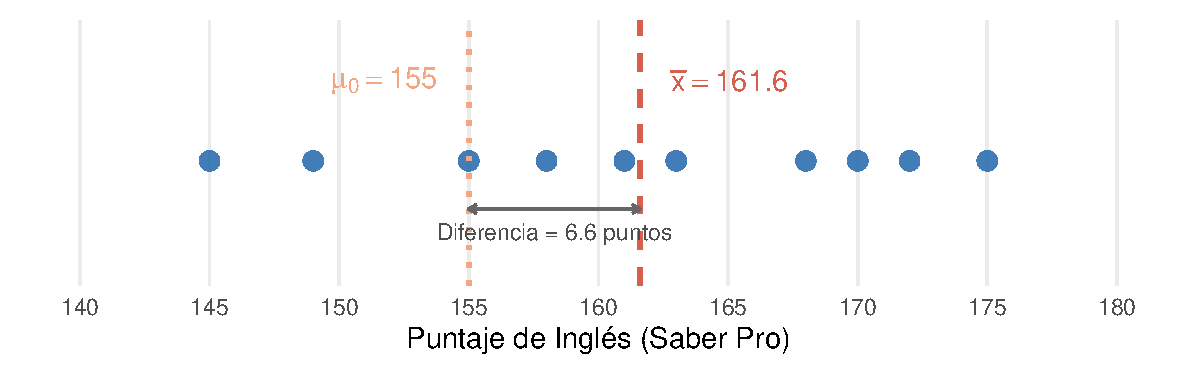
\includegraphics[width=0.85\textwidth]{S06_dotplot_repaso.pdf}
\end{center}

\begin{itemize}\setlength{\itemsep}{1pt}
  \item \textcolor{red}{\textbf{- -}} $\bar{x} = 161.6$ (nuestra muestra) \quad
  \textcolor{orange}{\textbf{$\cdots$}} $\mu_0 = 155$ (media nacional)
  \item Datos repartidos entre 145 y 175; diferencia de 6.6 puntos
\end{itemize}

\vspace{0.3cm}
\begin{block}{Observaci\'on visual}
$\bar{x}$ est\'a por encima de $\mu_0$, pero algunos datos caen \emph{por debajo} de 155. ?`La diferencia de 6.6 puntos es real o es solo variabilidad?
\end{block}
\end{frame}

% --- PASO 4: Distribución muestral ---
\begin{frame}{Paso 4: Distribuci\'on muestral y error est\'andar (S03)}
\small
Sabemos que $\bar{x}$ \textbf{var\'ia de muestra en muestra}. Si tom\'aramos otra muestra de 10 estudiantes, obtendr\'iamos otro $\bar{x}$.

\vspace{0.2cm}
\textbf{Error est\'andar}: mide cu\'anto var\'ia $\bar{x}$ por azar:
\[
\text{SE} = \frac{s}{\sqrt{n}} = \frac{9.96}{\sqrt{10}} = \frac{9.96}{3.162} = 3.15
\]

\begin{center}
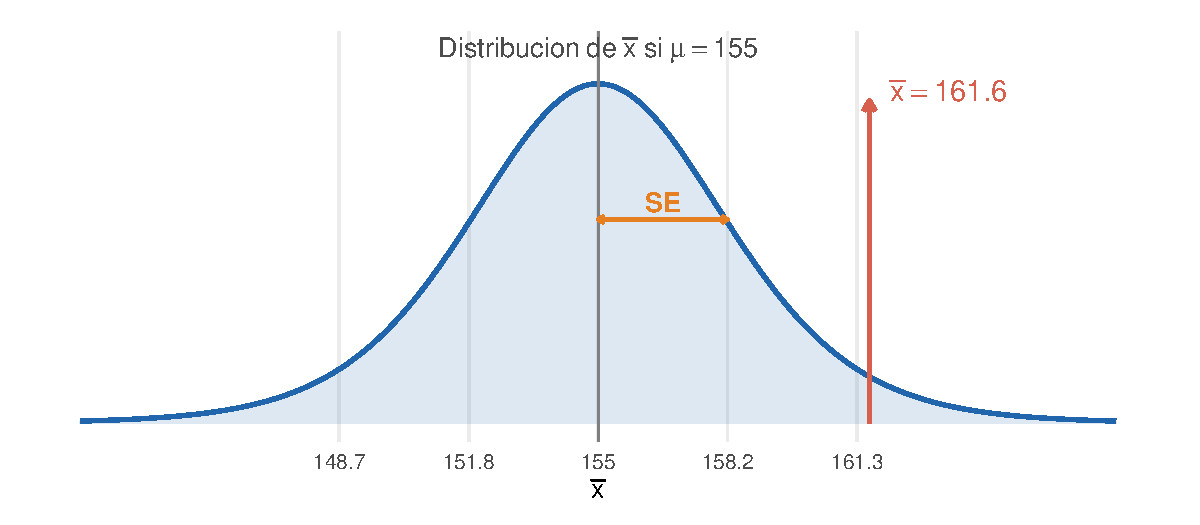
\includegraphics[width=\linewidth]{S06_dist_muestral.pdf}
\end{center}

$\bar{x} = 161.6$ est\'a a $\dfrac{161.6 - 155}{3.15} = 2.10$ errores est\'andar de $\mu_0$. ?`Es mucho?
\end{frame}

% --- PASO 5: IC ---
\begin{frame}{Paso 5: Intervalo de confianza al 95\% (S04)}
\small
Con $n = 10$, gl $= 9$, usamos $t_{0.025,\,9} = 2.262$:
\[
\text{IC}_{95\%} = \bar{x} \pm t_{0.025,9} \cdot \text{SE} = 161.6 \pm 2.262 \times 3.15 = 161.6 \pm 7.13
\]
\[
\boxed{\text{IC}_{95\%} = (154.47,\;\; 168.73)}
\]

\begin{center}
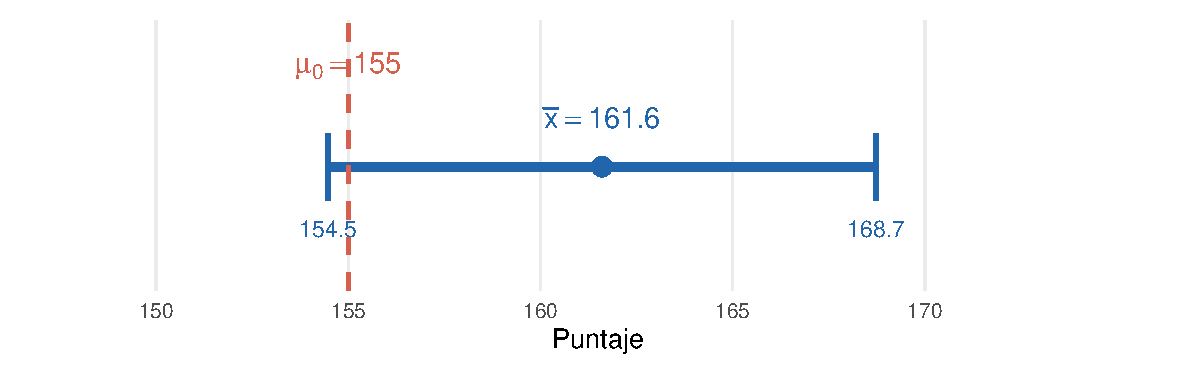
\includegraphics[width=\linewidth]{S06_ic_repaso.pdf}
\end{center}

\begin{block}{?`Qu\'e nos dice el IC?}
$\mu_0 = 155$ \alert{cae dentro} del IC $(154.5, 168.7)$. Esto significa que 155 es un valor \textbf{plausible} para la media poblacional. No podemos descartar que la universidad tenga la misma media que la nacional.
\end{block}
\end{frame}

% --- PASO 6: EL PROBLEMA ---
\begin{frame}{Paso 6: El problema --- ?`Y ahora qu\'e decidimos?}
\small

El rector dice: \emph{``Mis estudiantes superan la media nacional.''}

\vspace{0.3cm}
Con las herramientas de S01--S04, sabemos:
\begin{itemize}\setlength{\itemsep}{2pt}
  \item[\checkmark] $\bar{x} = 161.6 > 155$ (la muestra est\'a arriba)
  \item[\checkmark] Pero $\mu_0 = 155$ cae dentro del IC
  \item[\checkmark] La diferencia es de 2.10 errores est\'andar
\end{itemize}

\vspace{0.3cm}
\begin{alertblock}{Pero no podemos DECIDIR formalmente}
\begin{itemize}\setlength{\itemsep}{2pt}
  \item ?`Cu\'al es la probabilidad de ver $\bar{x} = 161.6$ si la media real \emph{fuera} 155?
  \item ?`Qu\'e tan confiados estamos en decir que la universidad es \textbf{mejor}?
  \item ?`Qu\'e riesgo corremos al equivocarnos?
\end{itemize}
\end{alertblock}

\vspace{0.2cm}
\centering
\textbf{Necesitamos un marco formal para tomar la decisi\'on.}\\
Eso es exactamente lo que son las \alert{pruebas de hip\'otesis}.
\end{frame}

% --- PASO 7: MOTIVACIÓN ---
\begin{frame}{?`Por qu\'e necesitamos pruebas de hip\'otesis?}
\small

\begin{columns}[T]
\column{0.48\textwidth}
\textbf{Lo que ya sabemos hacer:}
\begin{enumerate}\setlength{\itemsep}{2pt}
  \item[S01] Calcular $\bar{x}$, $s$, mediana
  \item[S02] Visualizar los datos
  \item[S03] Entender la variabilidad muestral
  \item[S04] Construir IC para $\mu$, $\sigma^2$, $p$
\end{enumerate}

\column{0.48\textwidth}
\textbf{Lo que \alert{NO} sabemos hacer:}
\begin{enumerate}\setlength{\itemsep}{2pt}
  \item Tomar una \textbf{decisi\'on} formal
  \item Cuantificar el \textbf{riesgo} de equivocarnos
  \item Distinguir se\~nal de \textbf{ruido}
  \item Medir si el efecto es \textbf{relevante}
\end{enumerate}
\end{columns}

\vspace{0.4cm}
\begin{exampleblock}{Hoy completamos el pipeline}
\centering
\small
Datos $\to$ Descriptivos $\to$ Visualizaci\'on $\to$ IC $\to$ \alert{Prueba de hip\'otesis} $\to$ \alert{Decisi\'on}
\end{exampleblock}

\vspace{0.2cm}
\textbf{Despu\'es de hoy}, con los mismos 10 datos podr\'as decir:\\
\emph{``Al 5\% de significancia, \textbf{no hay evidencia suficiente} para afirmar que la universidad supera la media nacional ($t = 2.10$, $p = 0.065$).''}
\end{frame}

% --- PARA QUÉ SIRVE ---
\begin{frame}{?`Para qu\'e sirven las pruebas de hip\'otesis?}
\small

\begin{center}
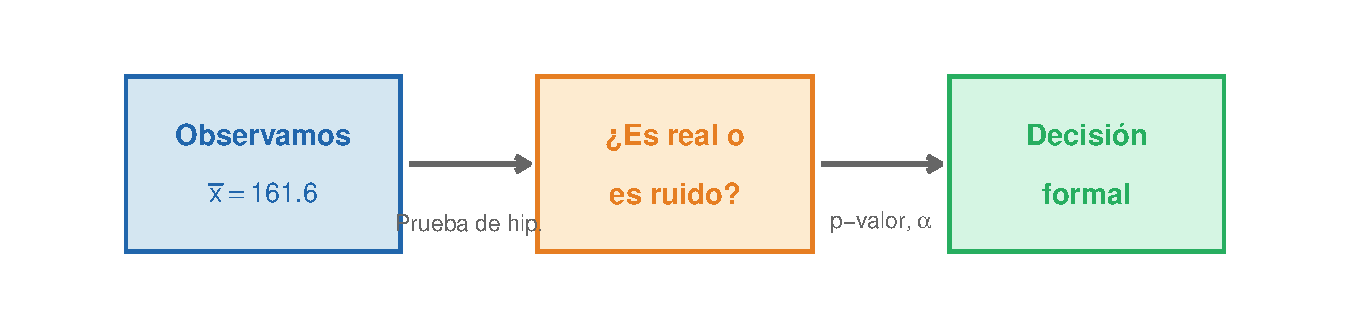
\includegraphics[width=\linewidth]{S06_flujo_hipotesis.pdf}
\end{center}

\vspace{0.2cm}
\textbf{Aplicaciones reales donde se usan cada d\'ia}:
\begin{itemize}\setlength{\itemsep}{3pt}
  \item \textbf{Medicina}: ?`El medicamento reduce la presi\'on arterial o es efecto placebo?
  \item \textbf{A/B testing}: ?`El bot\'on verde genera m\'as clics que el azul en la app?
  \item \textbf{Pol\'itica p\'ublica}: ?`El programa de becas mejor\'o los puntajes del ICFES?
  \item \textbf{Tu tesis/trabajo}: ?`Los datos soportan tu hip\'otesis de investigaci\'on?
\end{itemize}

\vspace{0.2cm}
\begin{block}{Mensaje clave}
Sin pruebas de hip\'otesis, cualquier afirmaci\'on sobre datos es \textbf{opini\'on}. Con ellas, es \textbf{evidencia cuantificada}.
\end{block}
\end{frame}

% ===================== INICIO S06 =====================
\begin{frame}{}
\vfill
\centering
{\Large\textbf{Sesi\'on 6}}\\[1em]
{\normalsize Fundamentos de Pruebas de Hip\'otesis}\\[0.5em]
{\small $H_0$, $H_1$, p-valor, errores y potencia estad\'istica}
\vfill
\end{frame}

% ============================================================================
\section{Introducción a las Pruebas de Hipótesis}
% ============================================================================

\begin{frame}{?`Por qu\'e aprender pruebas de hip\'otesis?}
\small
\begin{exampleblock}{Decisiones basadas en datos, no en intuici\'on}
\begin{itemize}\setlength{\itemsep}{2pt}
  \item \textbf{Spotify}: ?`Realmente los usuarios escuchan m\'as m\'usica con el nuevo algoritmo de recomendaciones, o fue casualidad?
  \item \textbf{Rappi}: ?`El nuevo dise\~no de la app aumenta los pedidos, o la diferencia es solo ruido aleatorio?
  \item \textbf{Tu futuro trabajo}: ``Jefe, los datos muestran que la campa\~na funcion\'o'' --- ?`c\'omo lo demuestras formalmente?
\end{itemize}
\end{exampleblock}

\vspace{0.2cm}
Las pruebas de hip\'otesis son el marco formal para tomar \alert{decisiones} con datos. No basta con ``parece que s\'i''; necesitas cuantificar qu\'e tan seguro est\'as.
\end{frame}

\begin{frame}{¿Qué es una Hipótesis Estadística?}
\begin{definition}[Hipótesis estadística]
Una \textbf{hipótesis estadística} es una afirmación sobre un parámetro poblacional que puede ser verdadera o falsa.
\end{definition}

\vspace{0.2cm}
\textbf{Ejemplos}:
\begin{itemize}
  \item La media de ingl\'es en NI es 160 puntos ($\mu = 160$)
  \item La proporci\'on que supera B1 es mayor al 70\% ($p > 0.70$)
  \item IES p\'ublicas y privadas tienen el mismo rendimiento ($\mu_1 = \mu_2$)
\end{itemize}

\vspace{0.1cm}
\textbf{Diferencia con IC}: el IC estima un rango plausible para $\mu$; la prueba de hip\'otesis pregunta si hay evidencia suficiente para afirmar que $\mu \neq 160$.

\begin{exampleblock}{Ejemplo cercano}
¿Los que escuchan lofi realmente estudian m\'as horas? $H_0$: no hay diferencia. $H_1$: s\'i hay diferencia.
\end{exampleblock}
\end{frame}

\begin{frame}{Hipótesis Nula vs Hipótesis Alternativa}
\begin{columns}[T]
\column{0.48\textwidth}
\begin{block}{Hipótesis nula ($H_0$)}
\begin{itemize}
  \item Se asume verdadera inicialmente
  \item ``No diferencia'' o ``no efecto''
  \item Contiene igualdad: $=$, $\leq$, $\geq$
  \item Buscamos \alert{rechazarla} con evidencia
\end{itemize}
\end{block}

\column{0.48\textwidth}
\begin{block}{Hipótesis alternativa ($H_1$ o $H_a$)}
\begin{itemize}
  \item La afirmación que queremos probar
  \item Refleja el interés de investigación
  \item Contiene: $\neq$, $<$, o $>$
  \item Solo la aceptamos con \alert{evidencia fuerte}
\end{itemize}
\end{block}
\end{columns}

\vspace{0.3cm}
\textbf{Analogía jurídica}: $H_0$ = ``inocente'', $H_1$ = ``culpable''. Asumimos inocencia hasta que se pruebe culpabilidad.
\end{frame}

\begin{frame}{Tres Formas de la Hipótesis Alternativa}
\textbf{1. Prueba de dos colas (bilateral)}:
\[
H_0: \mu = \mu_0 \quad \text{vs} \quad H_1: \mu \neq \mu_0
\]
\textbf{Pregunta}: ¿Es $\mu$ \alert{diferente} de $\mu_0$ (mayor O menor)?

\vspace{0.3cm}
\textbf{2. Prueba de cola derecha (unilateral)}:
\[
H_0: \mu \leq \mu_0 \quad \text{vs} \quad H_1: \mu > \mu_0
\]
\textbf{Pregunta}: ¿Es $\mu$ \alert{mayor} que $\mu_0$?

\vspace{0.3cm}
\textbf{3. Prueba de cola izquierda (unilateral)}:
\[
H_0: \mu \geq \mu_0 \quad \text{vs} \quad H_1: \mu < \mu_0
\]
\textbf{Pregunta}: ¿Es $\mu$ \alert{menor} que $\mu_0$?

\vspace{0.3cm}
\textbf{Nota}: La forma depende de la pregunta de investigación.
\end{frame}

\begin{frame}{Ejemplos con Datos ICFES}
\textbf{Ejemplo 1 (dos colas)}: ¿El puntaje promedio de inglés en NI es diferente de 160?
\[
H_0: \mu = 160 \quad \text{vs} \quad H_1: \mu \neq 160
\]

\vspace{0.3cm}
\textbf{Ejemplo 2 (cola derecha)}: ¿El puntaje promedio de inglés en NI supera el umbral de B1 (160)?
\[
H_0: \mu \leq 160 \quad \text{vs} \quad H_1: \mu > 160
\]

\vspace{0.3cm}
\textbf{Ejemplo 3 (cola izquierda)}: ¿El puntaje promedio de matemáticas en NI es inferior a 150?
\[
H_0: \mu \geq 150 \quad \text{vs} \quad H_1: \mu < 150
\]

\vspace{0.3cm}
\textbf{Decisión}: Depende del contexto y la pregunta. Si no hay razón para esperar una dirección específica, usar dos colas.
\end{frame}

\begin{frame}{La Hipótesis Nula como ``Statu Quo''}
\textbf{Filosofía}:
\begin{itemize}
  \item $H_0$ representa el estado actual del conocimiento o la creencia aceptada
  \item Solo la rechazamos si los datos muestran evidencia \alert{fuerte} en contra
  \item Si no hay evidencia suficiente, mantenemos $H_0$ (NO la "aceptamos")
\end{itemize}

\vspace{0.3cm}
\textbf{Ejemplos}:
\begin{itemize}
  \item $H_0$: "El nuevo método de enseñanza NO mejora el rendimiento" (statu quo)
  \item $H_1$: "El nuevo método SÍ mejora el rendimiento" (afirmación que queremos probar)
\end{itemize}

\vspace{0.3cm}
\begin{alertblock}{Importante}
\textbf{No rechazar $H_0$} NO es lo mismo que "aceptar $H_0$". Solo significa que no hay evidencia suficiente para rechazarla. Puede ser que:
\begin{itemize}
  \item $H_0$ sea verdadera
  \item La muestra sea muy pequeña (falta de poder estadístico)
\end{itemize}
\end{alertblock}
\end{frame}

\begin{frame}{Analogía con un Juicio}
\begin{center}
\begin{tabular}{lcl}
\textbf{Juicio} & & \textbf{Prueba de hipótesis} \\[0.3cm]
Acusado & $\longleftrightarrow$ & Hipótesis nula $H_0$ \\
Inocente (presunción) & $\longleftrightarrow$ & $H_0$ es verdadera (presunción) \\
Evidencia & $\longleftrightarrow$ & Datos de la muestra \\
Veredicto "culpable" & $\longleftrightarrow$ & Rechazar $H_0$ \\
Veredicto "no culpable" & $\longleftrightarrow$ & No rechazar $H_0$ \\
\end{tabular}
\end{center}

\vspace{0.5cm}
\textbf{Principio clave}: Solo declaramos "culpable" (rechazamos $H_0$) si la evidencia es \alert{más allá de una duda razonable}.

\vspace{0.3cm}
\textbf{Nota}: "No culpable" $\neq$ "inocente". Solo significa que no hay evidencia suficiente para condenar.
\end{frame}

% ============================================================================
\section{Error Tipo I, Tipo II y Nivel de Significancia}
% ============================================================================

\begin{frame}{?`Por qu\'e aprender sobre errores estad\'isticos?}
\small
\begin{exampleblock}{Equivocarse tiene costos reales}
\begin{itemize}\setlength{\itemsep}{2pt}
  \item \textbf{App de citas}: el algoritmo dice que hay ``match perfecto'' pero no lo hay (falso positivo). O dice que no hay match cuando s\'i lo hay (falso negativo).
  \item \textbf{Netflix}: recomendar una serie que no te gusta (error tipo I) vs.\ no recomendarte una que te encantar\'ia (error tipo II).
  \item \textbf{Antifraude bancario}: bloquear tu tarjeta sin raz\'on vs.\ no detectar un fraude real.
\end{itemize}
\end{exampleblock}

\vspace{0.2cm}
En estad\'istica, \alert{siempre} hay riesgo de equivocarse. Lo importante es entender y controlar ese riesgo.
\end{frame}

\begin{frame}{Dos Tipos de Errores}
\textbf{Decisiones posibles}:
\begin{enumerate}
  \item Rechazar $H_0$
  \item No rechazar $H_0$
\end{enumerate}

\vspace{0.3cm}
\textbf{Realidad desconocida}:
\begin{enumerate}
  \item $H_0$ es verdadera
  \item $H_0$ es falsa
\end{enumerate}

\vspace{0.3cm}
Esto da lugar a 4 escenarios:
\begin{table}
\centering
\small
\begin{tabular}{lcc}
\toprule
& \textbf{$H_0$ verdadera} & \textbf{$H_0$ falsa} \\
\midrule
\textbf{No rechazar $H_0$} & Decisión correcta & \textcolor{red}{Error tipo II ($\beta$)} \\
\textbf{Rechazar $H_0$} & \textcolor{red}{Error tipo I ($\alpha$)} & Decisión correcta \\
\bottomrule
\end{tabular}
\end{table}
\end{frame}

\begin{frame}{Error Tipo I ($\alpha$)}
\begin{definition}[Error tipo I]
Rechazar $H_0$ cuando en realidad es \alert{verdadera}.
\end{definition}

\vspace{0.2cm}
\begin{itemize}
  \item También llamado \textbf{falso positivo}
  \item Probabilidad: $P(\text{rechazar } H_0 \mid H_0 \text{ verdadera}) = \alpha$
  \item En la analogía jurídica: condenar a un inocente
\end{itemize}

\vspace{0.2cm}
\textbf{Ejemplo educativo}: $H_0$: ``El nuevo programa NO mejora el rendimiento''. Error tipo I: concluir que funciona cuando no tiene efecto. Consecuencia: invertir recursos en un programa inefectivo.

\begin{exampleblock}{Ejemplo Gen Z}
Declarar que un producto es \textit{viral} en TikTok cuando no lo es (falso positivo en marketing). Una marca invierte millones en algo que ``todos quieren'' pero nadie compra.
\end{exampleblock}
\end{frame}

\begin{frame}{Error Tipo II ($\beta$)}
\begin{definition}[Error tipo II]
\alert{No rechazar} $H_0$ cuando en realidad es \alert{falsa}.
\end{definition}

\vspace{0.2cm}
\begin{itemize}
  \item También llamado \textbf{falso negativo}
  \item Probabilidad: $P(\text{no rechazar } H_0 \mid H_0 \text{ falsa}) = \beta$
  \item En la analogía jurídica: absolver a un culpable
\end{itemize}

\vspace{0.2cm}
\textbf{Ejemplo educativo}: $H_0$: ``El programa NO mejora el rendimiento''. Error tipo II: concluir que no funciona cuando s\'i mejora. Consecuencia: descartar un programa efectivo.

\begin{exampleblock}{Ejemplo Gen Z}
Tu emprendimiento lanza un anuncio en Instagram que realmente atrae clientes, pero con solo 15 respuestas concluyes que ``no sirve'' y lo cancelas (falso negativo).
\end{exampleblock}
\end{frame}

\begin{frame}{Tabla Resumen de Errores}
\begin{table}
\centering
\small
\begin{tabular}{p{2.8cm}p{3.8cm}p{3.8cm}}
\toprule
\textbf{Escenario} & \textbf{Error tipo I ($\alpha$)} & \textbf{Error tipo II ($\beta$)} \\
\midrule
\textbf{Definición} & Rechazar $H_0$ verdadera & No rechazar $H_0$ falsa \\[0.15cm]
\textbf{Nombre alternativo} & Falso positivo & Falso negativo \\[0.15cm]
\textbf{Analogía jurídica} & Condenar inocente & Absolver culpable \\[0.15cm]
\textbf{Analogía médica} & Diagnóstico positivo en sano & Diagnóstico negativo en enfermo \\[0.15cm]
\textbf{Control} & Fijamos $\alpha$ (0.05, 0.01) & Depende de $n$, $\alpha$, efecto \\
\bottomrule
\end{tabular}
\end{table}
\end{frame}

\begin{frame}{Nivel de Significancia $\alpha$}
\begin{definition}[Nivel de significancia]
El \textbf{nivel de significancia} $\alpha$ es la probabilidad máxima de cometer un error tipo I que estamos dispuestos a tolerar.
\end{definition}

\vspace{0.2cm}
\textbf{Valores comunes}:
\begin{itemize}
  \item $\alpha = 0.05$ (5\%): estándar en ciencias sociales
  \item $\alpha = 0.01$ (1\%): cuando queremos ser más conservadores
  \item $\alpha = 0.10$ (10\%): cuando el error tipo II es más costoso
\end{itemize}

\vspace{0.2cm}
\textbf{Interpretación}: Con $\alpha = 0.05$, aceptamos que en el 5\% de las pruebas (a largo plazo) rechazaremos $H_0$ incorrectamente.

\begin{alertblock}{Importante}
$\alpha$ NO es la probabilidad de que $H_0$ sea verdadera. Es la probabilidad de rechazarla \alert{si} es verdadera.
\end{alertblock}
\end{frame}

\begin{frame}{Trade-off entre $\alpha$ y $\beta$}
\textbf{Relación inversa}:
\begin{itemize}
  \item Si reducimos $\alpha$ (ser más estrictos para rechazar $H_0$), aumenta $\beta$
  \item Si aumentamos $\alpha$ (ser menos estrictos), disminuye $\beta$
\end{itemize}

\vspace{0.3cm}
\begin{center}
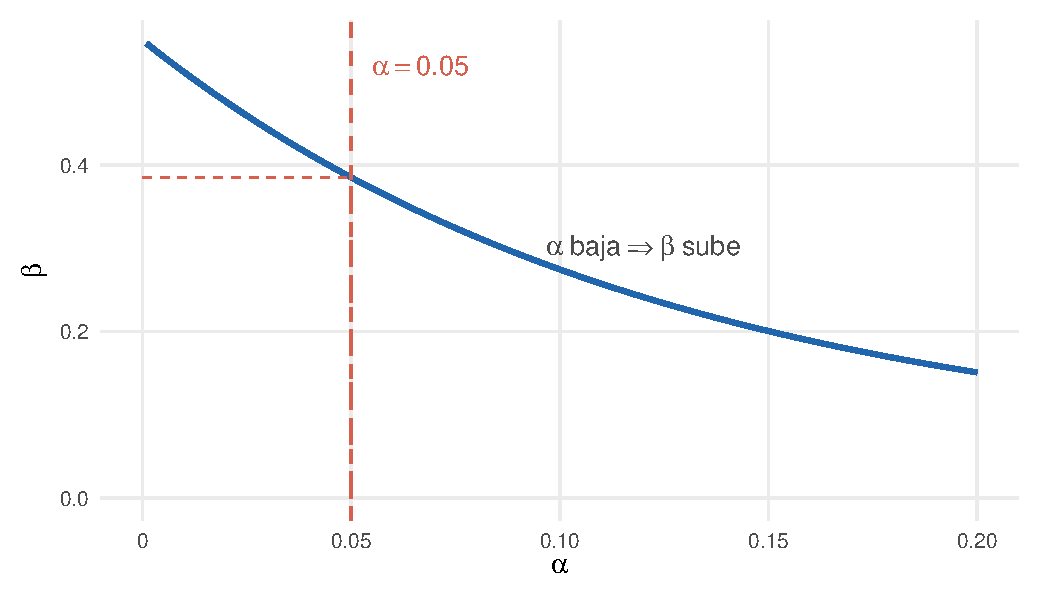
\includegraphics[width=0.75\linewidth]{S06_tradeoff_alpha_beta.pdf}
\end{center}

\vspace{0.3cm}
\textbf{Solución}: Aumentar el tamaño de muestra $n$ reduce TANTO $\alpha$ como $\beta$.
\end{frame}

% ============================================================================
\section{El p-valor}
% ============================================================================

\begin{frame}{?`Por qu\'e aprender sobre el p-valor?}
\small
\begin{exampleblock}{El n\'umero m\'as citado (y malinterpretado) de la ciencia}
\begin{itemize}\setlength{\itemsep}{2pt}
  \item Cada vez que lees ``el estudio es estad\'isticamente significativo'' en noticias, redes o papers, est\'an hablando del p-valor.
  \item Empresas como Google, Meta y Amazon toman decisiones de millones de d\'olares basadas en p-valores de A/B tests.
  \item Si vas a trabajar con datos, \alert{necesitas} saber qu\'e significa y qu\'e NO significa.
\end{itemize}
\end{exampleblock}

\vspace{0.2cm}
El p-valor es una herramienta poderosa, pero mal usada lleva a conclusiones err\'oneas. Vamos a entenderlo bien.
\end{frame}

\begin{frame}{¿Qué es el p-valor?}
\begin{definition}[p-valor]
El \textbf{p-valor} es la probabilidad de obtener un resultado tan extremo o más extremo que el observado, \alert{asumiendo que $H_0$ es verdadera}.
\end{definition}

\vspace{0.2cm}
\textbf{Fórmula conceptual}:
\[
\text{p-valor} = P(\text{estadístico tan extremo o más} \mid H_0 \text{ verdadera})
\]

\textbf{Interpretación}:
\begin{itemize}
  \item p-valor \alert{pequeño} $\Rightarrow$ datos incompatibles con $H_0$ $\Rightarrow$ evidencia contra $H_0$
  \item p-valor \alert{grande} $\Rightarrow$ datos compatibles con $H_0$ $\Rightarrow$ no hay evidencia contra $H_0$
\end{itemize}

\begin{block}{Regla de decisión}
Si p-valor $< \alpha$, rechazamos $H_0$.\\
Si p-valor $\geq \alpha$, no rechazamos $H_0$.
\end{block}
\end{frame}

\begin{frame}{El p-valor: ejemplo concreto}
\begin{exampleblock}{Ejemplo}
Si comparas horas de estudio entre quienes escuchan lofi y quienes no, y el p-valor es 0.03, hay solo un 3\% de probabilidad de ver una diferencia tan grande \alert{si realmente no hubiera diferencia}. Como $0.03 < 0.05$, rechazamos $H_0$.
\end{exampleblock}

\vspace{0.3cm}
\textbf{Recordar}: El p-valor solo mide evidencia contra $H_0$, no prueba que $H_1$ sea verdadera.
\end{frame}

\begin{frame}{Errores Comunes de Interpretación del p-valor}
\begin{alertblock}{Lo que el p-valor NO es}
\begin{enumerate}
  \item \textcolor{red}{\textbf{NO}} es $P(H_0 \text{ verdadera} \mid \text{datos})$
  \begin{itemize}
    \item Es al revés: $P(\text{datos} \mid H_0 \text{ verdadera})$
  \end{itemize}

  \item \textcolor{red}{\textbf{NO}} es la probabilidad de que el resultado sea "por azar"
  \begin{itemize}
    \item Todo en estadística involucra azar; el p-valor cuantifica qué tan compatible son los datos con $H_0$
  \end{itemize}

  \item \textcolor{red}{\textbf{NO}} mide la magnitud del efecto
  \begin{itemize}
    \item Un p-valor pequeño puede deberse a un efecto pequeño con muestra grande
  \end{itemize}

  \item \textcolor{red}{\textbf{NO}} es la probabilidad de replicar el resultado
\end{enumerate}
\end{alertblock}
\end{frame}

\begin{frame}{Escala Cualitativa del p-valor}
\begin{table}
\centering
\begin{tabular}{lll}
\toprule
\textbf{p-valor} & \textbf{Evidencia contra $H_0$} & \textbf{Decisión ($\alpha = 0.05$)} \\
\midrule
$p < 0.01$ & Muy fuerte & Rechazar $H_0$ \\
$0.01 \leq p < 0.05$ & Moderada & Rechazar $H_0$ \\
$0.05 \leq p < 0.10$ & Débil & No rechazar $H_0$ \\
$p \geq 0.10$ & Ninguna & No rechazar $H_0$ \\
\bottomrule
\end{tabular}
\end{table}

\vspace{0.3cm}
\textbf{Notas}:
\begin{itemize}
  \item Esta es una guía general, no una regla rígida
  \item El umbral de 0.05 es convencional, no mágico
  \item En algunos campos (física de partículas), se usa $\alpha = 0.0000003$ (5 sigmas)
  \item En estudios exploratorios, a veces se tolera $\alpha = 0.10$
\end{itemize}
\end{frame}

\begin{frame}{Visualización del p-valor (dos colas)}
\begin{center}
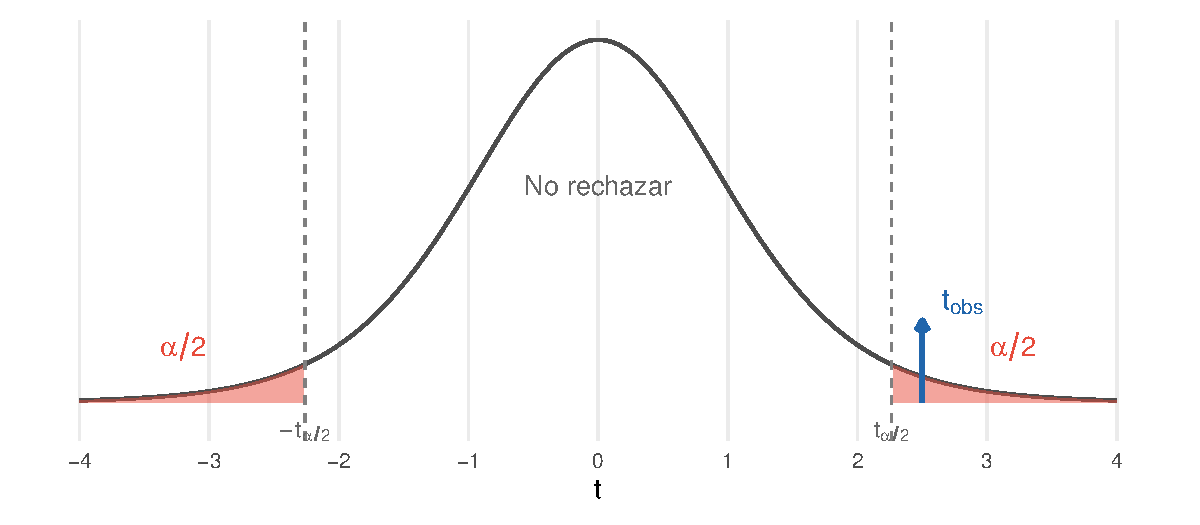
\includegraphics[width=\linewidth]{S06_pvalor_dos_colas.pdf}
\end{center}

\vspace{0.3cm}
\small
p-valor = área en rojo MÁS ALLÁ de $|t_{\text{obs}}|$ (ambas colas).\\
Si p-valor $< \alpha$, $t_{\text{obs}}$ cae en la región de rechazo.
\end{frame}

% ============================================================================
\section{Prueba z para una Muestra ($\sigma$ Conocida)}
% ============================================================================

\begin{frame}{?`Por qu\'e aprender la prueba $z$?}
\small
\begin{exampleblock}{Tu primera herramienta de decisi\'on}
Imagina que Spotify dice: ``nuestros usuarios escuchan en promedio 90 minutos al d\'ia''. T\'u encuestas a 200 usuarios colombianos y obtienes $\bar{x} = 82$ minutos. ?`Es una diferencia real o solo variabilidad muestral?
\end{exampleblock}

\vspace{0.2cm}
La prueba $z$ es el caso m\'as simple: comparar una media muestral contra un valor te\'orico cuando conocemos $\sigma$. Es el punto de partida para entender todas las dem\'as pruebas.

\vspace{0.2cm}
\begin{block}{En la pr\'actica}
Casi nunca conocemos $\sigma$ (por eso luego veremos la prueba $t$), pero la prueba $z$ nos da la \alert{l\'ogica fundamental} que subyace a todas las pruebas de hip\'otesis.
\end{block}
\end{frame}

\begin{frame}{Estadístico de Prueba $z$}
\textbf{Supuestos}:
\begin{itemize}
  \item Muestra aleatoria simple de tamaño $n$
  \item Población normal O $n \geq 30$ (TLC)
  \item $\sigma$ conocida
\end{itemize}

\vspace{0.3cm}
\begin{block}{Estadístico de prueba}
\[
z = \frac{\bar{x} - \mu_0}{\sigma / \sqrt{n}}
\]
donde:
\begin{itemize}
  \item $\mu_0$ = valor hipotético de $H_0: \mu = \mu_0$
  \item Si $H_0$ es verdadera, $z \sim N(0,1)$
\end{itemize}
\end{block}

\vspace{0.3cm}
\textbf{Interpretación}: $z$ mide cuántas desviaciones estándar está $\bar{x}$ del valor hipotético $\mu_0$.
\end{frame}

\begin{frame}{Región de Rechazo y Valor Crítico}
\textbf{Prueba de dos colas}: $H_0: \mu = \mu_0$ vs $H_1: \mu \neq \mu_0$
\begin{itemize}
  \item Rechazar $H_0$ si $|z| > z_{\alpha/2}$
  \item p-valor = $2 \cdot P(Z > |z_{\text{obs}}|)$
\end{itemize}

\vspace{0.3cm}
\textbf{Prueba de cola derecha}: $H_0: \mu \leq \mu_0$ vs $H_1: \mu > \mu_0$
\begin{itemize}
  \item Rechazar $H_0$ si $z > z_{\alpha}$
  \item p-valor = $P(Z > z_{\text{obs}})$
\end{itemize}

\vspace{0.3cm}
\textbf{Prueba de cola izquierda}: $H_0: \mu \geq \mu_0$ vs $H_1: \mu < \mu_0$
\begin{itemize}
  \item Rechazar $H_0$ si $z < -z_{\alpha}$
  \item p-valor = $P(Z < z_{\text{obs}})$
\end{itemize}
\end{frame}

\begin{frame}{Ejemplo paso a paso: ?`La media de ingl\'es supera 155? (prueba $z$)}
\small
\textbf{Datos}: $n = 120$, $\bar{x} = 162.5$, $\sigma = 18$ (conocida), $\mu_0 = 155$, $\alpha = 0.05$.

\textbf{Hip\'otesis}: $H_0: \mu \leq 155$ \quad vs \quad $H_1: \mu > 155$ (cola derecha)

\vspace{0.2cm}
\textbf{Paso 1 --- Error est\'andar}:
\[
\text{SE} = \frac{\sigma}{\sqrt{n}} = \frac{18}{\sqrt{120}} = \frac{18}{10.95} = 1.643
\]

\textbf{Paso 2 --- Estad\'istico $z$}:
\[
z = \frac{\bar{x} - \mu_0}{\text{SE}} = \frac{162.5 - 155}{1.643} = \frac{7.5}{1.643} = 4.56
\]

\textbf{Paso 3 --- Comparar con valor cr\'itico}: $z_{0.05} = 1.645$
\[
4.56 > 1.645 \quad \Rightarrow \quad \alert{\text{Rechazamos } H_0}
\]

\textbf{Conclusi\'on}: Hay evidencia muy fuerte de que $\mu > 155$.
\end{frame}

% ============================================================================
\section{Prueba t para una Muestra ($\sigma$ Desconocida)}
% ============================================================================

\begin{frame}{?`Por qu\'e aprender la prueba $t$?}
\small
\begin{exampleblock}{La prueba que realmente vas a usar}
En la vida real, \alert{nunca} conoces la desviaci\'on est\'andar poblacional $\sigma$. Cuando encuestas a tus compa\~neros sobre horas de sue\~no, calculas $s$ de tu muestra, no de toda la poblaci\'on. La prueba $t$ est\'a dise\~nada exactamente para eso.
\end{exampleblock}

\vspace{0.2cm}
\textbf{Diferencia pr\'actica}:
\begin{itemize}\setlength{\itemsep}{1pt}
  \item Prueba $z$: necesitas $\sigma$ (casi nunca la tienes)
  \item Prueba $t$: usas $s$ (siempre la puedes calcular)
  \item Con $n$ grande, dan resultados pr\'acticamente iguales
\end{itemize}

\vspace{0.1cm}
La prueba $t$ es la herramienta est\'andar para la gran mayor\'ia de situaciones pr\'acticas.
\end{frame}

\begin{frame}{Estad\'istico de Prueba $t$}
\textbf{Caso real}: $\sigma$ desconocida, usamos $s$.

\vspace{0.3cm}
\begin{block}{Estad\'istico de prueba}
\[
t = \frac{\bar{x} - \mu_0}{s / \sqrt{n}}, \quad \text{gl} = n - 1
\]
Si $H_0$ es verdadera, $t \sim t(n-1)$. Se compara con la \textbf{tabla de valores cr\'iticos}.
\end{block}

\vspace{0.3cm}
\textbf{Regiones de rechazo}:
\begin{itemize}
  \item \textbf{Dos colas}: Rechazar si $|t| > t_{\alpha/2,\; n-1}$
  \item \textbf{Cola derecha}: Rechazar si $t > t_{\alpha,\; n-1}$
  \item \textbf{Cola izquierda}: Rechazar si $t < -t_{\alpha,\; n-1}$
\end{itemize}
\end{frame}

\begin{frame}{Ejemplo paso a paso: prueba $t$ con nuestros 10 datos del repaso}
\small
\textbf{Retomamos los datos del repaso}: $n = 10$, $\bar{x} = 161.6$, $s = 9.96$, $\mu_0 = 155$.

\textbf{Hip\'otesis}: $H_0: \mu = 155$ \quad vs \quad $H_1: \mu \neq 155$ (bilateral, $\alpha = 0.05$)

\vspace{0.2cm}
\textbf{Paso 1 --- Error est\'andar}:
$\text{SE} = s/\sqrt{n} = 9.96/\sqrt{10} = 9.96/3.162 = 3.15$

\textbf{Paso 2 --- Estad\'istico $t$}:
$t = (\bar{x} - \mu_0)/\text{SE} = (161.6 - 155)/3.15 = 6.6/3.15 = 2.10$

\textbf{Paso 3 --- Valor cr\'itico}: gl $= 9$, $t_{0.025,\,9} = 2.262$

\textbf{Paso 4 --- Decisi\'on}:
$|2.10| = 2.10 < 2.262 \quad \Rightarrow \quad$ \textbf{No rechazamos $H_0$}

\vspace{0.2cm}
\begin{alertblock}{Conclusi\'on}
Al 5\%, \textbf{no hay evidencia suficiente} para afirmar que la universidad tiene media diferente de 155. La diferencia de 6.6 puntos podr\'ia ser variabilidad muestral con solo 10 estudiantes.
\end{alertblock}
\end{frame}

\begin{frame}{Conexi\'on: el IC ya nos lo dec\'ia}
\small

Recordemos del repaso: IC$_{95\%} = (154.47,\; 168.73)$.

\vspace{0.2cm}
\begin{center}
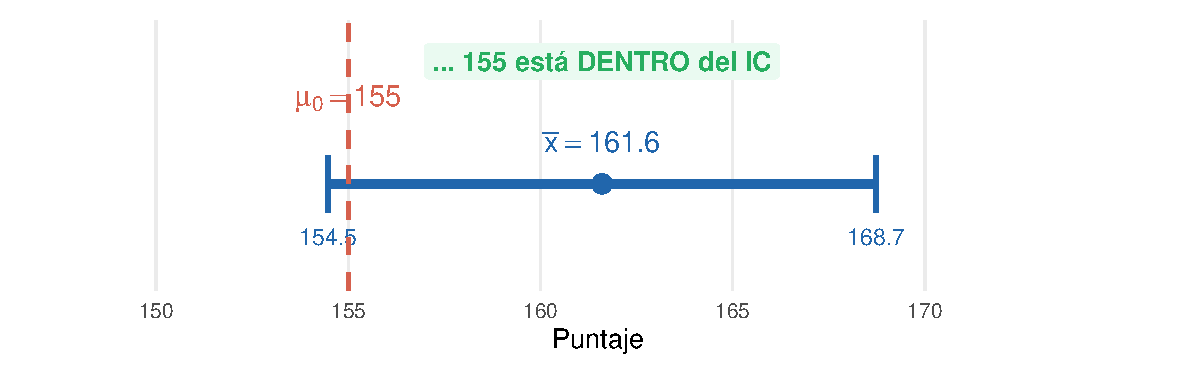
\includegraphics[width=\linewidth]{S06_ic_conexion.pdf}
\end{center}

\begin{block}{Equivalencia IC $\leftrightarrow$ Prueba bilateral}
\begin{itemize}\setlength{\itemsep}{2pt}
  \item $\mu_0 = 155$ cae \textbf{dentro} del IC al 95\% $\Rightarrow$ No rechazamos $H_0$ al 5\%
  \item $|t| = 2.10 < t_{0.025,9} = 2.262$ $\Rightarrow$ No rechazamos $H_0$ al 5\%
  \item \alert{Misma conclusi\'on}: dos formas de ver lo mismo
\end{itemize}
\end{block}
\end{frame}

\begin{frame}{?`Y si la prueba fuera unilateral?}
\small
El rector dice que sus estudiantes \textbf{superan} la media nacional. Eso es una hip\'otesis direccional:

$H_0: \mu \leq 155$ \quad vs \quad $H_1: \mu > 155$ (cola derecha, $\alpha = 0.05$)

\vspace{0.2cm}
\textbf{Mismo estad\'istico}: $t = 2.10$

\textbf{Valor cr\'itico unilateral}: $t_{0.05,\,9} = 1.833$

\textbf{Decisi\'on}: $2.10 > 1.833$ $\Rightarrow$ \alert{Rechazamos $H_0$}

\vspace{0.3cm}
\begin{alertblock}{Ojo: la conclusi\'on cambi\'o}
\begin{itemize}
  \item Bilateral ($t_{0.025} = 2.262$): No rechaza
  \item Unilateral ($t_{0.05} = 1.833$): \textbf{S\'i rechaza}
\end{itemize}
La elecci\'on de bilateral vs.\ unilateral \textbf{importa}. Debe definirse \emph{antes} de ver los datos, seg\'un la pregunta de investigaci\'on.
\end{alertblock}
\end{frame}

% ============================================================================
\section{Prueba t para Dos Muestras Independientes}
% ============================================================================

\begin{frame}{?`Por qu\'e aprender a comparar dos grupos?}
\small
\begin{exampleblock}{La pregunta m\'as natural del mundo}
\begin{itemize}\setlength{\itemsep}{2pt}
  \item ?`Los estudiantes de universidades privadas sacan mejor puntaje en ingl\'es que los de p\'ublicas?
  \item ?`Los usuarios de iPhone gastan m\'as en apps que los de Android?
  \item ?`Las mujeres duermen m\'as horas que los hombres en semana de parciales?
\end{itemize}
\end{exampleblock}

\vspace{0.2cm}
Comparar dos grupos es una de las preguntas m\'as frecuentes en investigaci\'on, marketing y pol\'itica p\'ublica. La prueba $t$ de dos muestras es la herramienta est\'andar.
\end{frame}

\begin{frame}{Comparar Dos Medias Poblacionales}
\textbf{Pregunta}: ¿Difiere el rendimiento promedio entre dos grupos?

\vspace{0.3cm}
\textbf{Ejemplos}:
\begin{itemize}
  \item ¿El puntaje de inglés difiere entre IES públicas y privadas?
  \item ¿El salario inicial promedio difiere entre hombres y mujeres en NI?
  \item ¿Estudiantes de Bogotá tienen mejor rendimiento que los de otras regiones?
\end{itemize}

\vspace{0.3cm}
\textbf{Hipótesis}:
\[
H_0: \mu_1 = \mu_2 \quad \text{vs} \quad H_1: \mu_1 \neq \mu_2
\]
(o $H_1: \mu_1 > \mu_2$ o $H_1: \mu_1 < \mu_2$)

\vspace{0.3cm}
\textbf{Equivalente}:
\[
H_0: \mu_1 - \mu_2 = 0 \quad \text{vs} \quad H_1: \mu_1 - \mu_2 \neq 0
\]
\end{frame}

\begin{frame}{Estadístico de Prueba para Dos Muestras}
\textbf{Supuestos}: Dos muestras aleatorias \alert{independientes}; poblaciones normales o $n_1, n_2 \geq 30$; varianzas desconocidas.

\vspace{0.2cm}
\begin{block}{Estadístico de prueba (Welch)}
\[
t = \frac{(\bar{x}_1 - \bar{x}_2) - 0}{\sqrt{\dfrac{s_1^2}{n_1} + \dfrac{s_2^2}{n_2}}}
\]
\end{block}

\vspace{0.2cm}
\textbf{Grados de libertad (Welch)}: \quad
$\text{gl} = \dfrac{\left(\frac{s_1^2}{n_1} + \frac{s_2^2}{n_2}\right)^2}{\frac{(s_1^2/n_1)^2}{n_1-1} + \frac{(s_2^2/n_2)^2}{n_2-1}}$

\smallskip
\small No necesitas memorizarla; R la calcula automáticamente.
\end{frame}

\begin{frame}{Ejemplo paso a paso: Privadas vs.\ P\'ublicas en Bogot\'a}
\small
\textbf{Datos}:

\begin{center}
\begin{tabular}{lcccc}
\toprule
& $n$ & $\bar{x}$ & $s$ \\
\midrule
Privadas & 16 & 161 & 9 \\
P\'ublicas & 25 & 148 & 12 \\
\bottomrule
\end{tabular}
\end{center}

$H_0: \mu_1 = \mu_2$ \quad vs \quad $H_1: \mu_1 \neq \mu_2$ \quad ($\alpha = 0.05$)

\vspace{0.2cm}
\textbf{Paso 1 --- SE de la diferencia} (Welch):
\[
\text{SE} = \sqrt{\frac{s_1^2}{n_1} + \frac{s_2^2}{n_2}} = \sqrt{\frac{81}{16} + \frac{144}{25}} = \sqrt{5.0625 + 5.76} = \sqrt{10.82} = 3.29
\]

\textbf{Paso 2 --- Estad\'istico $t$}:
$t = \dfrac{161 - 148}{3.29} = \dfrac{13}{3.29} = 3.95$

\textbf{Paso 3} --- gl $\approx 39$, $t_{0.025,\,39} = 2.023$

\textbf{Decisi\'on}: $|3.95| > 2.023$ $\Rightarrow$ \alert{Rechazamos $H_0$}. Hay diferencia significativa.
\end{frame}

\begin{frame}{IC para la diferencia y verificaci\'on}
\small
\textbf{IC al 95\% para $\mu_1 - \mu_2$}:
\[
(\bar{x}_1 - \bar{x}_2) \pm t_{0.025,\,39} \cdot \text{SE} = 13 \pm 2.023 \times 3.29 = 13 \pm 6.66
\]
\[
\boxed{\text{IC}_{95\%} = (6.34,\;\; 19.66)}
\]

\vspace{0.2cm}
\begin{block}{Verificaci\'on de equivalencia}
\begin{itemize}
  \item El IC \textbf{no contiene al 0} $\Rightarrow$ Rechazamos $H_0: \mu_1 = \mu_2$
  \item El estad\'istico $|t| = 3.95 > 2.023$ $\Rightarrow$ Rechazamos $H_0$
  \item \alert{Misma conclusi\'on}: los estudiantes de privadas tienen en promedio entre 6.3 y 19.7 puntos m\'as que los de p\'ublicas
\end{itemize}
\end{block}

\vspace{0.2cm}
\textbf{Pero\ldots} ?`es esa diferencia \emph{grande} o \emph{peque\~na}? Para eso necesitamos medir el \textbf{tama\~no del efecto}.
\end{frame}

% ============================================================================
\section{d de Cohen y Tamaño del Efecto}
% ============================================================================

\begin{frame}{?`Por qu\'e aprender sobre tama\~no del efecto?}
\small
\begin{exampleblock}{Significativo $\neq$ importante}
\begin{itemize}\setlength{\itemsep}{2pt}
  \item Con 10 millones de usuarios, Netflix puede detectar que un bot\'on rojo genera 0.01\% m\'as clics que uno azul. Es ``significativo'' estad\'isticamente, pero ?`vale la pena cambiar el dise\~no?
  \item Si comparas notas entre dos universidades con 50{,}000 estudiantes y la diferencia es de 0.2 puntos sobre 500\ldots\ ?`es relevante?
\end{itemize}
\end{exampleblock}

\vspace{0.2cm}
El p-valor te dice \textbf{si} hay diferencia. El tama\~no del efecto te dice \textbf{cu\'anto importa} esa diferencia. Necesitas ambos para tomar buenas decisiones.
\end{frame}

\begin{frame}{Significancia Estadística vs Significancia Práctica}
\textbf{Problema}: Con muestras grandes, diferencias muy pequeñas pueden ser estadísticamente significativas (p-valor pequeño) pero \alert{irrelevantes} en la práctica.

\vspace{0.3cm}
\textbf{Ejemplo}:
\begin{itemize}
  \item $n_1 = n_2 = 10{,}000$
  \item $\bar{x}_1 = 162.5$, $\bar{x}_2 = 161.8$ (diferencia de 0.7 puntos)
  \item p-valor $< 0.001$ (muy significativo estadísticamente)
  \item ¿Es relevante una diferencia de 0.7 puntos en inglés?
\end{itemize}

\vspace{0.3cm}
\begin{alertblock}{Lección}
\textbf{Significancia estadística} (p-valor pequeño) $\neq$ \textbf{Significancia práctica} (efecto relevante).

\vspace{0.2cm}
Necesitamos medir el \alert{tamaño del efecto}.
\end{alertblock}
\end{frame}

\begin{frame}{d de Cohen}
\begin{definition}[d de Cohen]
Una medida estandarizada del tamaño del efecto:
\[
d = \frac{\bar{x}_1 - \bar{x}_2}{s_{\text{pooled}}} \qquad \text{donde } s_{\text{pooled}} = \sqrt{\frac{(n_1 - 1)s_1^2 + (n_2 - 1)s_2^2}{n_1 + n_2 - 2}}
\]
\end{definition}

\vspace{0.2cm}
\textbf{Interpretación (Cohen, 1988)}:
\begin{itemize}
  \item $|d| \approx 0.2$: efecto \alert{pequeño} \quad $|d| \approx 0.5$: efecto \alert{mediano} \quad $|d| \approx 0.8$: efecto \alert{grande}
\end{itemize}

\vspace{0.2cm}
\textbf{Ventaja}: Independiente del tamaño de muestra y de las unidades de medida.
\end{frame}

\begin{frame}{Calcular $d$ de Cohen paso a paso}
\small
Continuando con privadas ($n_1 = 16$, $s_1 = 9$) vs.\ p\'ublicas ($n_2 = 25$, $s_2 = 12$):

\vspace{0.2cm}
\textbf{Paso 1 --- Desviaci\'on est\'andar pooled}:
\[
s_p = \sqrt{\frac{(n_1-1)s_1^2 + (n_2-1)s_2^2}{n_1+n_2-2}} = \sqrt{\frac{15 \times 81 + 24 \times 144}{39}} = \sqrt{\frac{1215 + 3456}{39}} = \sqrt{\frac{4671}{39}} = \sqrt{119.8} = 10.94
\]

\textbf{Paso 2 --- $d$ de Cohen}:
\[
d = \frac{|\bar{x}_1 - \bar{x}_2|}{s_p} = \frac{|161 - 148|}{10.94} = \frac{13}{10.94} = \boxed{1.19}
\]

\vspace{0.2cm}
\begin{block}{Interpretaci\'on}
\begin{itemize}
  \item $d = 1.19$ es un efecto \alert{grande} ($> 0.8$)
  \item La diferencia entre privadas y p\'ublicas es de 1.19 desviaciones est\'andar
  \item Diferencia estad\'isticamente significativa \textbf{Y} pr\'acticamente relevante
\end{itemize}
\end{block}
\end{frame}

\begin{frame}{Reporte Completo: Estadística + Efecto}
\textbf{Recomendación}: Siempre reportar TANTO la significancia estadística como el tamaño del efecto.

\vspace{0.3cm}
\begin{exampleblock}{Ejemplo de reporte}
``Se encontró una diferencia estadísticamente significativa en el puntaje promedio de inglés entre estudiantes de IES públicas ($M = 160.3$, $DE = 17.8$) y privadas ($M = 166.5$, $DE = 18.2$), $t(238) = -2.41$, $p = 0.017$, $d = 0.35$. Aunque la diferencia es significativa, el tamaño del efecto es pequeño.''
\end{exampleblock}

\vspace{0.3cm}
\textbf{Elementos clave}:
\begin{enumerate}
  \item Estadísticos descriptivos ($M$, $DE$)
  \item Estadístico de prueba ($t$) y gl
  \item p-valor
  \item Tamaño del efecto ($d$)
  \item Interpretación contextual
\end{enumerate}
\end{frame}

% ============================================================================
\section{Potencia Estadística}
% ============================================================================

\begin{frame}{?`Por qu\'e aprender sobre potencia estad\'istica?}
\small
\begin{exampleblock}{?`Tu estudio puede detectar algo?}
Imagina que haces una encuesta a 15 compa\~neros para ver si escuchar lofi mejora las notas. Encuentras que ``no hay diferencia significativa''. Pero\ldots\ ?`realmente no hay diferencia, o es que 15 personas son muy pocas para detectarla?
\end{exampleblock}

\vspace{0.2cm}
La \textbf{potencia} responde esta pregunta: ?`qu\'e tan capaz es tu estudio de encontrar un efecto \alert{si realmente existe}?

\vspace{0.2cm}
\begin{block}{Aplicaci\'on pr\'actica}
Antes de gastar tiempo y dinero recolectando datos, la potencia te dice cu\'antas observaciones necesitas. Es la diferencia entre un estudio \'util y uno que no puede concluir nada.
\end{block}
\end{frame}

\begin{frame}{¿Qué es la Potencia Estadística?}
\begin{definition}[Potencia estadística]
\[
\text{Potencia} = 1 - \beta = P(\text{rechazar } H_0 \mid H_0 \text{ falsa})
\]
Es la probabilidad de \alert{detectar} un efecto cuando realmente existe.
\end{definition}

\vspace{0.2cm}
\textbf{Interpretación}:
\begin{itemize}
  \item Alta potencia (ej. 0.80 o 80\%) = buena capacidad de detectar efectos reales
  \item Baja potencia (ej. 0.30) = es probable que NO detectemos un efecto aunque exista
\end{itemize}

\vspace{0.2cm}
\textbf{Convención}: Potencia m\'inima aceptable: 0.80 (80\%). Ideal: 0.90 o mayor.

\smallskip
\textit{Piens\'enlo as\'i}: la potencia es la capacidad de tu encuesta para detectar una diferencia real. Si encuestas a solo 10 personas sobre lofi y estudio, probablemente no detectar\'as nada aunque la diferencia exista.
\end{frame}

\begin{frame}{Factores que Afectan la Potencia}
\begin{enumerate}
  \item \textbf{Tamaño de muestra ($n$)}: Mayor $n$ $\Rightarrow$ mayor potencia

  \item \textbf{Nivel de significancia ($\alpha$)}: Mayor $\alpha$ $\Rightarrow$ mayor potencia (pero más error tipo I)

  \item \textbf{Tamaño del efecto}: Efectos grandes son más fáciles de detectar

  \item \textbf{Variabilidad ($\sigma$)}: Menor $\sigma$ $\Rightarrow$ mayor potencia
\end{enumerate}

\vspace{0.3cm}
\textbf{Relación clave}:
\[
\text{Potencia} = f(n, \alpha, \text{efecto}, \sigma)
\]

\vspace{0.3cm}
\textbf{Control}: El único factor que controlamos fácilmente es $n$ (diseño del estudio).
\end{frame}

\begin{frame}{Curva de Potencia}
\begin{center}
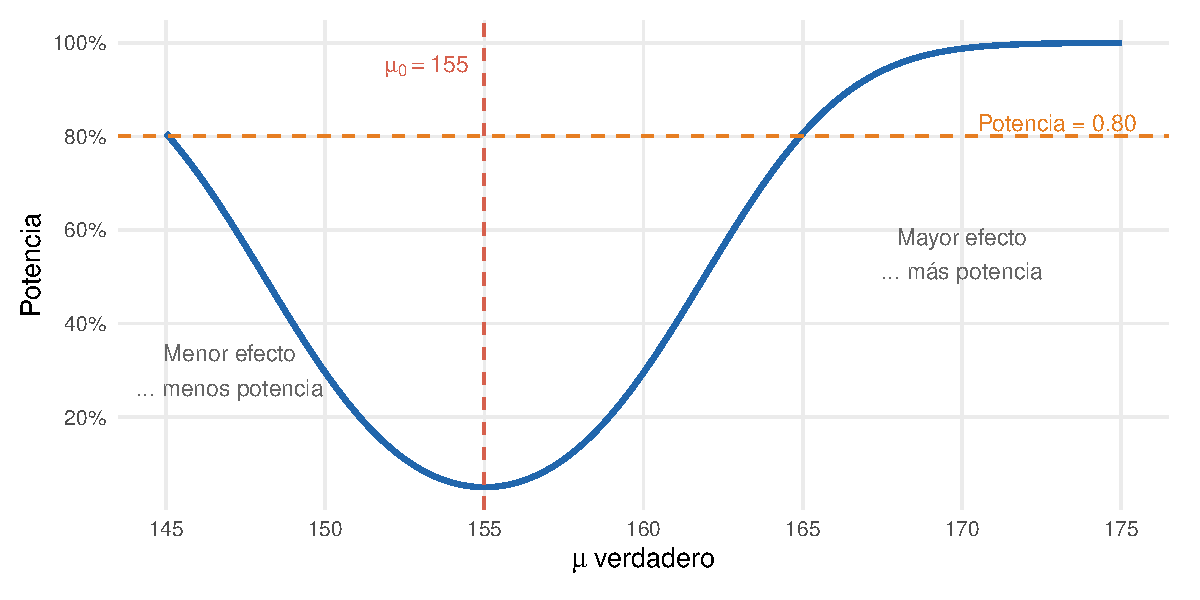
\includegraphics[width=0.85\linewidth]{S06_curva_potencia.pdf}
\end{center}

\vspace{0.3cm}
\small
La potencia aumenta cuando el verdadero $\mu$ se aleja más de $\mu_0$ (mayor tamaño del efecto).
\end{frame}

\begin{frame}{Potencia en la pr\'actica: ?`cu\'antos estudiantes necesito?}
\small
\textbf{Regla pr\'actica}: para detectar un efecto de tama\~no $d$ con potencia 0.80 y $\alpha = 0.05$ (dos colas), se necesita aproximadamente:

\vspace{0.2cm}
\begin{center}
\begin{tabular}{ccc}
\toprule
$d$ de Cohen & Tama\~no del efecto & $n$ aprox.\ por grupo \\
\midrule
0.2 & Peque\~no & 394 \\
0.3 & Peque\~no-mediano & 176 \\
0.5 & Mediano & 64 \\
0.8 & Grande & 26 \\
\bottomrule
\end{tabular}
\end{center}

\vspace{0.2cm}
\begin{alertblock}{Lecci\'on clave}
\begin{itemize}\setlength{\itemsep}{1pt}
  \item Efectos peque\~nos requieren muestras \textbf{enormes} para ser detectados
  \item Nuestro ejemplo del repaso ($n = 10$) tiene poca potencia para efectos peque\~nos
  \item \textbf{Antes de recolectar datos}, calcula cu\'antos necesitas
\end{itemize}
\end{alertblock}
\end{frame}

% ============================================================================
\section{Relación entre IC y Pruebas de Hipótesis}
% ============================================================================

\begin{frame}{?`Por qu\'e conectar IC con pruebas de hip\'otesis?}
\small
\begin{exampleblock}{Son dos formas de ver lo mismo}
En S05 construiste intervalos de confianza. Hoy aprendiste pruebas de hip\'otesis. Parece que son cosas distintas, pero en realidad son \alert{dos caras de la misma moneda}: si el valor hipot\'etico $\mu_0$ NO cae dentro del IC, entonces el p-valor es menor que $\alpha$.
\end{exampleblock}

\vspace{0.2cm}
\textbf{?`Por qu\'e importa?}
\begin{itemize}\setlength{\itemsep}{1pt}
  \item El IC te da m\'as informaci\'on: no solo dice ``hay diferencia'', sino \textbf{cu\'anto} podr\'ia ser la diferencia
  \item En reportes profesionales se recomienda presentar \alert{ambos}: IC + p-valor
  \item Entender la conexi\'on evita errores de interpretaci\'on
\end{itemize}
\end{frame}

\begin{frame}{Dos Caras de la Misma Moneda}
\begin{theorem}[Equivalencia IC - Prueba de hipótesis]
Si un IC al $(1-\alpha) \times 100\%$ para $\mu$ \alert{NO contiene} el valor $\mu_0$, entonces rechazamos $H_0: \mu = \mu_0$ al nivel de significancia $\alpha$ (prueba de dos colas).
\end{theorem}

\vspace{0.3cm}
\textbf{Ejemplo}:
\begin{itemize}
  \item IC al 95\% para $\mu$: $(162.3, 168.7)$
  \item $H_0: \mu = 160$ vs $H_1: \mu \neq 160$
  \item Como 160 NO está en el IC, rechazamos $H_0$ al 5\%
\end{itemize}

\vspace{0.3cm}
\textbf{Ventaja de los IC}:
\begin{itemize}
  \item Proporcionan más información que solo "rechazar/no rechazar"
  \item Muestran el rango de valores plausibles para $\mu$
  \item Facilitan la interpretación práctica
\end{itemize}
\end{frame}

\begin{frame}{Verificar la equivalencia: ejemplo visual}
\small

\begin{center}
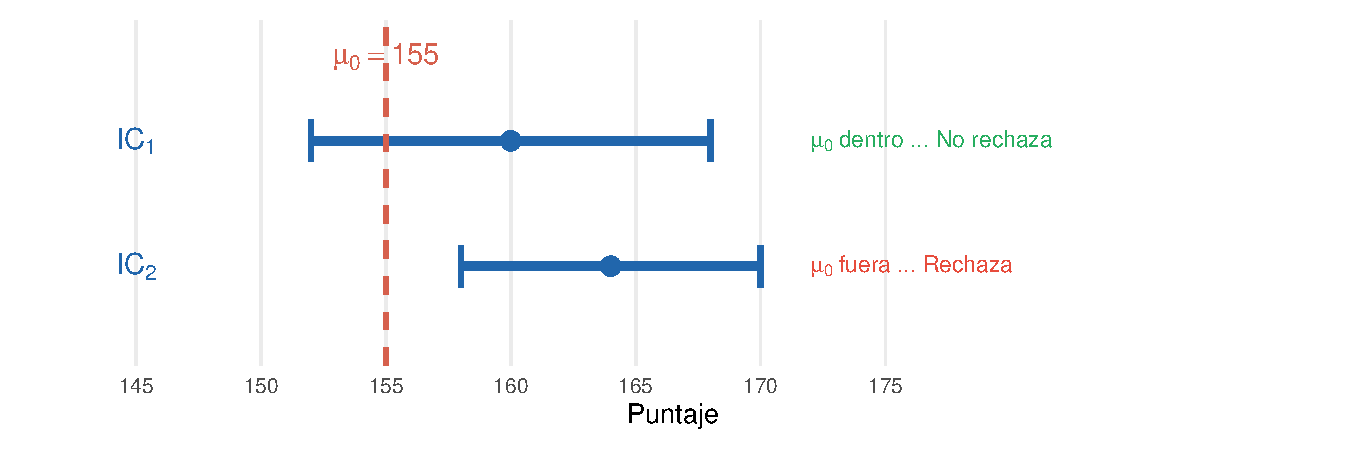
\includegraphics[width=\linewidth]{S06_ic_equivalencia.pdf}
\end{center}

\vspace{0.2cm}
\begin{block}{Regla}
\begin{itemize}
  \item $\mu_0$ \textbf{dentro} del IC al 95\% $\Leftrightarrow$ $|t| < t_{0.025}$ $\Leftrightarrow$ \textbf{No rechazar} $H_0$ al 5\%
  \item $\mu_0$ \textbf{fuera} del IC al 95\% $\Leftrightarrow$ $|t| > t_{0.025}$ $\Leftrightarrow$ \textbf{Rechazar} $H_0$ al 5\%
\end{itemize}
Siempre dan la \alert{misma conclusi\'on}. Son dos formas de ver lo mismo.
\end{block}
\end{frame}

\begin{frame}{¿Cuándo Usar IC vs Prueba de Hipótesis?}
\begin{columns}[T]
\column{0.48\textwidth}
\textbf{Intervalos de Confianza}:
\begin{itemize}
  \item Enfoque en \alert{estimación}
  \item ¿Cuál es el valor probable del parámetro?
  \item Proporcionan rango de valores
  \item Más informativos
  \item Útiles para reportar hallazgos
\end{itemize}

\column{0.48\textwidth}
\textbf{Pruebas de Hipótesis}:
\begin{itemize}
  \item Enfoque en \alert{decisión}
  \item ¿Hay evidencia contra $H_0$?
  \item Proporcionan p-valor
  \item Más formales
  \item Útiles para comparaciones
\end{itemize}
\end{columns}

\vspace{0.5cm}
\begin{exampleblock}{Recomendación}
En la práctica, \alert{reportar ambos}: IC + prueba de hipótesis. Esto da una visión completa de los resultados.
\end{exampleblock}
\end{frame}

% ============================================================================
\section{Conclusiones}
% ============================================================================

\begin{frame}{Resumen de la Sesión}
\textbf{Hoy aprendimos}:
\begin{enumerate}
  \item \textbf{Hipótesis}: $H_0$ (nula) vs $H_1$ (alternativa)
  \item \textbf{Errores}:
  \begin{itemize}
    \item Tipo I ($\alpha$): rechazar $H_0$ verdadera
    \item Tipo II ($\beta$): no rechazar $H_0$ falsa
  \end{itemize}
  \item \textbf{p-valor}: Probabilidad de datos tan extremos dado $H_0$ verdadera
  \item \textbf{Prueba z}: Para $\mu$ con $\sigma$ conocida
  \item \textbf{Prueba t}: Para $\mu$ con $\sigma$ desconocida (una muestra y dos muestras)
  \item \textbf{d de Cohen}: Medir tamaño del efecto
  \item \textbf{Potencia}: Probabilidad de detectar un efecto real
  \item \textbf{IC y pruebas}: Dos enfoques complementarios
\end{enumerate}

\vspace{0.3cm}
\textbf{Próxima sesión}: Prueba t pareada, ANOVA, y pruebas no paramétricas.
\end{frame}

\begin{frame}{Tabla Resumen: ¿Qué Prueba Usar?}
\begin{table}
\centering
\footnotesize
\begin{tabular}{p{3cm}p{2.5cm}p{4cm}}
\toprule
\textbf{Situación} & \textbf{Condición} & \textbf{Prueba} \\
\midrule
1 muestra, $\sigma$ conocida & $n$ grande o población normal & Prueba $z$ \\[0.2cm]
1 muestra, $\sigma$ desconocida & Población normal o $n \geq 30$ & Prueba $t$ (una muestra) \\[0.2cm]
2 muestras independientes & Poblaciones normales o $n_1, n_2 \geq 30$ & Prueba $t$ (dos muestras, Welch) \\[0.2cm]
2 muestras pareadas & Diferencias normales o $n \geq 30$ & Prueba $t$ pareada (próxima sesión) \\[0.2cm]
$> 2$ grupos & Normalidad, homocedasticidad & ANOVA (próxima sesión) \\
\bottomrule
\end{tabular}
\end{table}
\end{frame}

\begin{frame}{Ejercicios para practicar (a mano)}
\textbf{Resuelve paso a paso}:
\begin{enumerate}
  \item Con $n = 16$, $\bar{x} = 142$, $s = 16$: pruebe $H_0: \mu = 150$ vs $H_1: \mu \neq 150$ al 5\%. Calcule el IC al 95\% y verifique la equivalencia.
  \item Privadas: $n_1 = 36$, $\bar{x}_1 = 162$, $s_1 = 15$. P\'ublicas: $n_2 = 36$, $\bar{x}_2 = 152$, $s_2 = 18$. Pruebe $H_0: \mu_1 = \mu_2$ al 5\% y calcule el $d$ de Cohen.
  \item De $n = 400$ estudiantes, 140 obtuvieron B1+. Pruebe $H_0: p \geq 0.40$ vs $H_1: p < 0.40$ al 5\%.
  \item Con los datos del repaso ($n = 10$, $\bar{x} = 161.6$, $s = 9.96$), pruebe $H_0: \mu \leq 155$ vs $H_1: \mu > 155$ al 1\%. ?`Cambia la conclusi\'on respecto al 5\%?
\end{enumerate}

\vspace{0.3cm}
\begin{alertblock}{Preparaci\'on para el parcial}
Practiquen con el \textbf{banco de 30 ejercicios}. El examen tendr\'a 5 ejercicios del banco, todos para resolver a mano con tabla de valores cr\'iticos.
\end{alertblock}
\end{frame}

\begin{frame}
\begin{center}
\Large
¡Gracias por su atención!

\vspace{1cm}
\normalsize
Preguntas y discusión
\end{center}
\end{frame}

\end{document}
